\section{Notas} %

\begin{enumerate}
  
  \item Cuando se hacen comparaciones se toman los valores reales y se les restan los valores simulados $(Reales - \mathbb{E}[Simulados])$

  \item Para las simulaciones se utiliza la información anterior a la del semestre que se quiere simular para no tener información real dentro  de los datos para la simulación.
  
  \item Las matrices \textit{m\_grande} y de \textit{m\_grande\_total} tienen información real.
  
  \item El vector \textit{vec\_excepciones} tiene las posibles excepciones en las que las funciones que extraen información pueden caer, de esta manera se pueden generar nuevas funciones para corregir esos casos.
  
  \item La siguiente imagen es el resultado de la función \textit{imprime\_info\_idiomas} la cual muestra la información de los idiomas. Dicha función arroja un vector con los semestres que requieren modificación.

\begin{figure}[H]
\centering
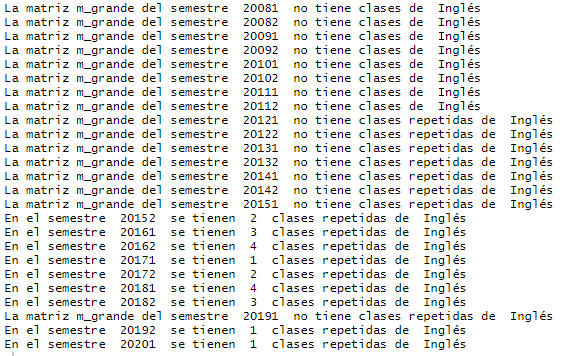
\includegraphics[scale = 0.8]{clases_de_ingles} %width=\textwidth
\caption{\textit{Resumen de clases de inglés antes de modificación}}
\end{figure}
  
Con esta información se decidió observar caso por caso los renglones que requieren modificación para la matriz \textit{m\_grande}


  \item Debido a la situación en la que estamos viviendo actualmente, ahora más que nunca es necesario tener un programa para la asignación de horarios. Que permita la realización de las asignaciones sin tener la necesidad de hacer reuniones en persona. Al proseguir con las medidas de distanciamiento social, las reuniones antiguamente hechas en persona se tendrían que hacer por medio de alguna plataforma digital. Éstas no necesariamente son las más óptimas ya que dependen de la señal de todos los participantes para que haya una comunicación de manera fluída. Debido a ésto, el programa es una buena solución.
  
  \item La información que se puede encontrar actualmente (debido a la pandemia) en las páginas web de los horarios de la Facultad no es la misma que la mostrada a lo largo del trabajo ya que ahora no se tiene información del salón, o del número de alumnos inscritos por materia, ni los lugares disponibles por grupo.
  
\begin{figure}[H]
\centering
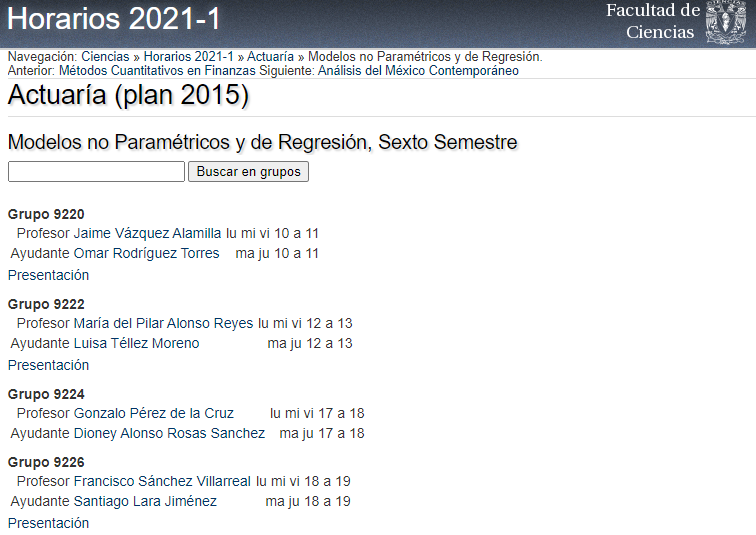
\includegraphics[scale = 0.7]{Ej_horarios_20211} %width=\textwidth
\caption{\textit{Ejemplo de horarios de semestre 2021-1}}
%\url{http://www.fciencias.unam.mx/docencia/horarios/20211/2017/1639}
\end{figure}
   
  \item La imagen \ref{img_en_ing_2} tiene título en inglés, se tienen 2 opciones: dejarlo así o buscar cómo cambiarlo.
   
  \item Arrigo dijo que posiblemente alguien se va a quejar de no tomar en cuenta la preferencia de los profesores al realizar las solicitudes.
  
  \item Cláusula 99 CCTPA: Ayuda para la impresión de la tesis.
  
  \url{https://www.personal.unam.mx/Docs/Contratos/AAPAUNAM20132015.pdf}

\begin{figure}[H]
\centering

\includegraphics[scale = 1]{clausula99_CCTPA} %width=\textwidth
\caption{\textit{Cláusula 99 CCTPA: Ayuda para la impresión de la tesis}}
\end{figure}
  
  \item La frecuencia relativa en los histogramas no refleja directamente el porcentaje. Se debe multiplicar el valor del eje $Y$ por el ancho del intervalo por $100$ para obtener cifras en porcentaje. El área total de las barras sumará 1 (\ref{MargaritaJaimeRuthLizbeth}).
  
  \item Las materias que se actualizaron o cambiaron de nombre se pueden ver en el Apéndice \ref{materias_agrupadas}.
  
	\item Arrigo dijo que posiblemente alguien se va a quejar del hecho de que actualmente las inscripciones ya no se hacen con tira de materias firmada.
  
  \item How to write your PhD thesis (without going insane) \url{https://www.youtube.com/watch?v=pM6orL-bGDc&ab_channel=JamesHaytonPhD}:
  
  \begin{itemize}
    \item Definir tiempos de trabajo y tiempos de trabajo.
  
  \item Ser constante. Escribir al menos una página al día.
  
  \item Escribir más de las áreas en las que se tiene mayor conocimiento que en temas que no se conocen al 100\%.
  
  \item Si se tiene un nivel de habilidad medio y el nivel del problema/reto es alto, entonces basta que uno se concentre en el problema para poder resolverlo.
  
\begin{figure}[H]
\centering
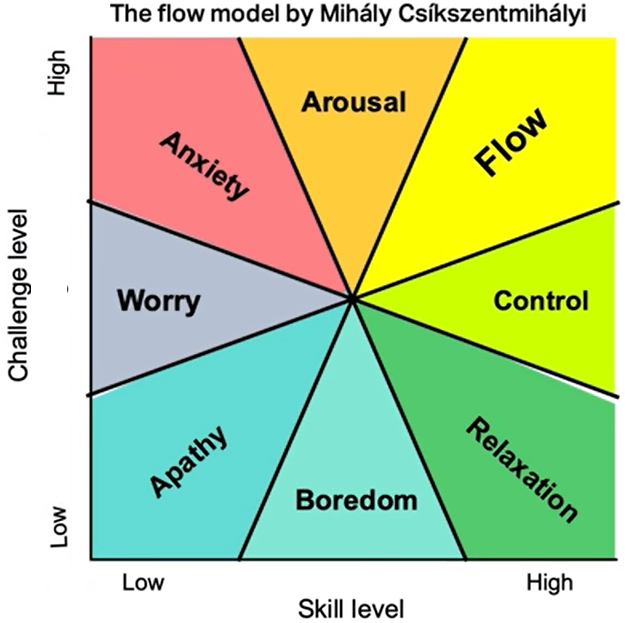
\includegraphics[scale = 0.65]{skill_vs_challenge_level} %width=\textwidth
\caption{\textit{Skill vs challenge level}}
\end{figure}  
  
  \end{itemize}
  
  \item Un programa de computadora, con que haga los mismos errores que un humano, es bueno porque su costo es menor.
    
  \item No se da 2 veces la misma materia al mismo profesor para que los alumnos tengan mayor gama de profesores para elegir.
    
  \item $X_{4}:$ Analizar presentación: Hacer varias pruebas con distintas combinaciones y elegir el mejor estilo/presentación.
  
  \item $X_{14}:$ Revisar/Investigar al respecto del problema y resolverlo.

\end{enumerate}
